
并发程序的开发通常挺难的,编写同时需要正确和高效(换句话说,所有这些都需要)的并发程序要困难得多。对于具有许多互斥对象或无锁的复杂性,会让编程更加困难。

管理这种复杂性的唯一方法就是进行封装,放入定义良好的代码或模块中。只要接口和需求是明确的,这些模块的使用者就不需要知道实现是无锁的还是基于锁的。它确实会影响性能,所以在优化之前,模块对于特定的需求可能不够用,但可以根据需要进行优化,而且这些优化仅限于特定的模块。

本章中将重点讨论为并发编程实现数据结构的模块。为什么是数据结构,而不是算法?首先,有很多关于并发算法的文献。其次,大多数开发者在处理算法上都有更宽裕的时间。分析代码,相应函数花费了过多的时间,再找到了一种不同的方法来实现算法,并在性能图表上移动到下一个高度。然后,最终会得到一个程序,其中没有一个单独的计算需要花费大量的时间,但仍然会有没有达到应有速度的感觉。原因:当没有热代码时,就可能有热数据。

数据结构在并发程序中扮演着更重要的角色,因为它们决定了如何保证算法的正确性,有哪些限制,和哪些并发操作可以安全执行?不同线程看到的数据视图是否一致?如果不知道这些问题的答案,就无法编写代码,而答案是由数据结构决定的。

与此同时,设计决策,比如接口和模块边界的选择,会对编写并发程序时的选择产生重大影响,并发不能作为事后的想法添加到设计中。在设计初始,就必须考虑到并发性,特别是数据的组织。

这里通过定义一些基本的术语和概念开始探索并发数据结构。

\subsubsubsection{6.4.1\hspace{0.2cm}并发数据结构的基础}

使用多线程的并发程序需要线程安全的数据结构。什么是线程安全?怎么使数据结构是线程安全的?乍一看,似乎很简单:如果一个数据结构可以被多个线程同时使用,并且没有任何数据竞争(在线程之间共享),那么它就是线程安全的。

然而,这个定义过于简单:

\begin{itemize}
\item 将标准定的很高——例如,没有一个STL容器是线程安全的。
\item 具有非常高的性能开销。
\item 这通常是不必要的,开销也是如此。
\item 在许多情况下完全没用。
\end{itemize}

我们将逐一解决这些问题。为什么线程安全的数据结构即使在多线程程序中也是不必要的?一种微小的可能性是,用于程序的单线程部分。我们努力最小化这些部分,因为它们对总体运行时间具有负面影响(还记得Amdahl定律吗?),但是大多数程序都有一些需要单线程处理的事情,使这些代码更快的方法是只做必要的事情。更常见的不需要线程安全的情况是,即使是在多线程程序中,一个对象仅由一个线程使用。这非常常见,也是非常可取的,共享数据是并发程序中效率低下的主要原因,因此可以尝试在每个线程上只使用本地对象和数据,独立地完成尽可能多的工作。

但是,即使每个对象永远不会在线程之间共享,能确定在多线程程序中使用一个类或一个数据结构是安全的吗?这还真不一定。仅在接口层没有看到共享,并不意味着在实现层没有。多个对象可以在内部共享相同的数据,静态成员和内存分配器只是其中的可能(我们倾向于认为所有需要内存的对象都通过调用\texttt{malloc()}获得,并且\texttt{malloc()}是线程安全的,而且类也可以实现自己的分配器)。

另一方面,只要没有线程修改对象,在多线程代码中使用许多数据结构是安全的。但必须再次考虑实现,接口可以是只读的,但实现仍然是可以修改对象。如果认为这是一种奇异的可能性,请考虑标准的C++共享指针\texttt{std::shared\_ptr}。当复制一个共享指针时,复制的对象不会修改,至少不会可见(通过\texttt{const}引用传递给新指针的构造函数)。与此同时,知道对象中的引用计数必须增加,这意味着复制的对象已经改变(在此场景中,共享指针是线程安全的,但这不是偶然,也不是免费的,同样也有性能成本)。

这里需要一个更细致的线程安全定义。但对于这个普遍的概念,没有通用的标准,不过有几个流行的版本。线程安全的最高级别通常称为\textbf{强线程安全保证},提供这种保证的对象可以被多个线程并发使用,而不会引起数据竞争或其他未定义的行为(特别是,任何不变量都会保留)。下一级称为\textbf{弱线程安全保证},只要所有线程都限制为只读访问(调用类的\texttt{const}成员函数),提供这种对象就可以使用多个线程同时访问。其次,任何对对象具有独占访问权的线程都可以对对象执行其他的操作(无论其他线程在同一时间做什么)。不提供任何此类保证的对象,不能在多线程程序中使用。即使对象本身不共享,其实现内部的某些内容也很容易被其他线程修改。

本书中,将使用强弱线程安全的语言保证。提供强担保的类有时简单地称为\textbf{线程安全}。只提供弱保证,则称为\textbf{线程兼容}。大多数STL容器都提供了这样的保证,若容器是一个线程的局部对象,可以以有效的方式使用,但若容器对象是共享的,只能调用\texttt{const}成员函数。最后,根本不提供任何保证的类称为\textbf{线程敌对},并且不能在多线程程序中使用。

实践中,经常遇到强保证和弱保证的组合。接口的一个子集提供强保证,其余部分只提供弱保证。

为什么不尝试在设计每个对象时都有强线程安全保证呢?第一个原因是,会有性能开销。保证通常是不必要的,因为对象不是在线程之间共享的,编写高效程序的关键是不做无用的工作。更有趣的反对意见是,即使在以需要线程安全的方式共享对象,强线程安全保证可能没用。假如需要开发一款玩家招募军队并进行战斗的游戏。军队中所有单位的名称都存储在一个容器中,比如一个字符串列表。另一个容器存储每个单元的当前强度。在战役中,单位总是会被杀死或招募,游戏引擎是多线程的,需要有效地管理庞大的军队。虽然STL容器只提供弱线程安全保证,但假设有一个强线程安全容器库。这是不够的,添加一个单元需要将它的名称插入到一个容器中,并将初始强度插入到另一个容器中,这两个操作本身都是线程安全的。一个线程创建一个新单元并将其插入到第一个容器中。在这个线程可以添加它的强度值之前,另一个线程看到这个新单位并需要查找它的强度,但是在第二个容器中还没有任何东西。问题在于线程安全的保证是在错误的层面上提供的。从应用程序的角度来看,创建新单元是一个事务,所有游戏引擎线程都应该能够在添加单元之前或之后查看数据库,但不能在中间状态。可以通过使用互斥锁来实现,在单元添加前锁定,只有在两个容器都新之后才会解锁。在这个场景中,只要这些对象的所有访问都由互斥锁保护,就不用关心单个容器提供的线程安全保证。显然,这里需要的是一个单元数据库,其本身提供所需的线程安全保证,例如:通过使用互斥对象。这个数据库可能在内部使用几个容器对象,数据库的实现可能需要或不需要这些容器的线程安全保证,但这对数据库的使用者应该是不可见的(拥有线程安全的容器可能会使实现更容易,也可能不会)。

这让我们得出一个非常重要的结论:线程安全始于设计阶段。必须明智地选择程序使用的数据结构和接口,以便表示适当的抽象级别,以及发生线程交互级别上的正确事务。

考虑到这一点,本章的其余部分应该从两个方面来看:一方面,展示如何设计和实现一些基本的线程安全的数据结构,这些数据结构可以用在程序中,构建更复杂(和更多样化)的构建块。另一方面,还展示了构建线程安全类的基本技术,这些类可用于设计更复杂的数据结构。

\subsubsubsection{6.4.2\hspace{0.2cm}计数器和累加器}

最简单的线程安全对象是简单的计数器或累加器,计数器只是计算在线程上可能发生的一些事件。所有线程都可能需要修改计数器或访问当前值,因此存在竞争条件。

弱线程安全保证无法满足我们的要求,这里需要强线程安全保证,从而确保读取没有更改的值总是线程安全的。我们已经看到了实现的可用选项:某种锁、原子操作(当有原子操作时)或无锁CAS循环。

锁的性能因实现的不同而不同,通常首选自旋锁。没有立即访问计数器的线程的等待时间将非常短,因此将线程置于睡眠状态,并在稍后将其唤醒所需的成本根本没有必要。另一方面,由于忙等待(轮询自旋锁)而浪费的CPU时间可以忽略不计,很可能只需要几条指令。

原子指令提供了良好的性能,但操作的选择相当有限。在C++中,可以原子地对整数进行加法,但不能对整数进行乘法。这对于简单的计数器来说已经足够了,但是对于累加器来说可能还不够(累加操作可能有多个结果)。如果有一种方法可用,肯定没有原子操作那么简单。

CAS循环可用于实现累加器,而不考虑需要使用的操作。然而,在大多数现代硬件上,性能比自旋锁的性能更好(参见图6.2),但不是最快的选择。

当使用自旋锁访问单个变量或单个对象时,可以进一步优化自旋锁。可以让锁成为保护对象的唯一引用,而不是通用标志。原子变量是指针,而不是整数。除此之外,锁定机制保持不变。因为\texttt{lock()}函数返回指向计数器的指针,所以是非标准的:

\hspace*{\fill} \\ %插入空行
\noindent
\textbf{01d\_ptrlock\_count.C}
\begin{lstlisting}[style=styleCXX]
template <typename T>
class PtrSpinlock {
	public:
	explicit PtrSpinlock(T* p) : p_(p) {}
	T* lock() {
		while (!(saved_p_ =
		p_.exchange(nullptr, std::memory_order_acquire))) {}
	}
	void unlock() {
		p_.store(saved_p_, std::memory_order_release);
	}
	private:
	std::atomic<T*> p_;
	T* saved_p_ = nullptr;
};
\end{lstlisting}

与之前的自旋锁实现相比,原子变量的含义“颠倒”了。如果原子变量\texttt{p\_}不为空,则该锁可用,否则为空。为自旋锁做的所有优化在这里也适用,看起来完全相同,所以不打算重复。另外,这个类需要一组删除复制的操作(锁是不可复制的)。如果需要转移锁,并将其释放给另一个对象,则该锁可以移动。如果锁拥有它所指向的对象,析构函数应该删除它(这结合了自旋锁和单类中unique指针的功能)。

指针自旋锁的第一个优点,提供了访问保护对象的唯一方式。这就不可能有条件竞争,并在没有锁的情况下访问共享数据。第二个优点,锁的性能通常略优于常规自旋锁,自旋锁是否优于原子操作也取决于硬件。相同的基准测试在不同的处理器上会出现不同的结果:

%\hspace*{\fill} \\ %插入空行
\begin{center}
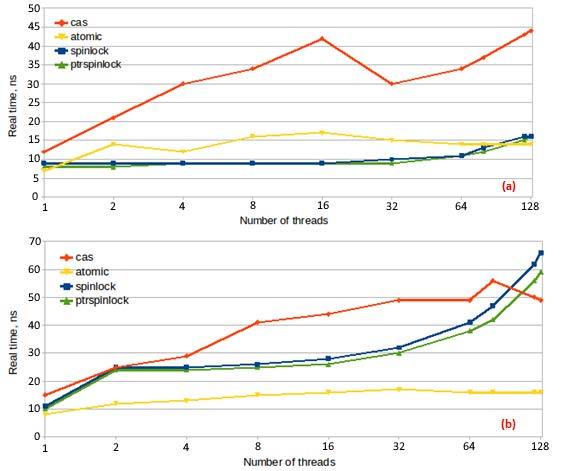
\includegraphics[width=0.9\textwidth]{content/2/chapter6/images/3.jpg}\\
图6.3 - 共享计数增量的性能:不同硬件系统(a)和(b)的常规自旋锁、指针自旋锁、无锁(比较-交换,或CAS)和无等待(原子)
\end{center}

通常,越新的处理器处理锁和忙等待的性能越好,而且自旋锁在最新的硬件上提供的性能也越好(图6.3中,系统\textit{b}使用的Intel x86 CPU比系统\textit{a}的CPU晚一代)。

执行一个操作所需的平均时间(或者相反的,吞吐量)是我们在大多数HPC系统中主要关注的指标。然而,这并不是用来衡量并发程序性能的唯一指标。如果程序在移动设备上运行,那么功耗可能更重要。所有线程使用的CPU总时间根据平均功耗的进行调整。用于测试计数器增量平均实时时间的基准测试,同样也可以用来测试CPU时间:

%\hspace*{\fill} \\ %插入空行
\begin{center}
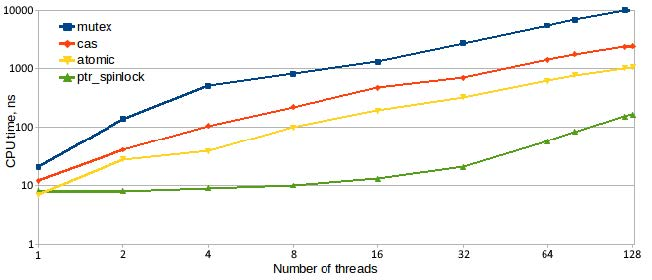
\includegraphics[width=0.9\textwidth]{content/2/chapter6/images/4.jpg}\\
图6.4 - 线程安全的计数器——不同实现使用的平均CPU时间
\end{center}

坏消息是,无论采用哪种实现,多个线程同时访问共享数据的成本都会随着线程数量的增加呈指数增长,至少在有很多线程的情况下是这样的(注意,图6.4中的y轴比例是对数的)。然而,不同的实现之间的效率差别很大,对于最高效的实现来说,在8个线程之后才会出现指数级的增长。注意,不同硬件系统的结果也会有所不同,所以必须根据目标平台进行选择,并且只有在完成测试后才能选择。

无论选择何种实现,线程安全的累加器或计数器都不应将其公开,而应将其封装在类中。原因之一是为类的客户端提供稳定的接口,同时保留优化实现的自由度。

第二个原因更微妙,与计数器提供的保证有关。目前,关注的是计数器本身,确保所有线程都可以对其进行修改和访问,而不存在任何竞争。这是否足够使用,取决于如何使用计数器。如果只是计算一些不依赖于计数器的值,那么只关心值本身是否正确就好。另一方面,如果计数的是数组中的元素数量,那么处理的就是数据依赖关系。假设有一个大型的预分配数组(或者一个容器,可以在不影响现有元素的情况下增长),所有线程都在计算要插入到这个数组中的新元素。计数器对进行计算的元素进行计数,并将值插入数组,可以由其他线程使用。若一个线程从计数器中读取值N,必须确保数组的前N个元素可以安全读取(这意味着没有其他线程修改它们)。但是数组本身既不是原子的,也不受锁的保护。可以通过锁来保护对整个数组的访问,但这可能会降低程序的性能。如果数组中已经有很多元素了,只有一个线程可以读取它们,那么程序就可能是单线程的。另一方面,从多个线程读取常量、不可变数据都是安全的,不需要任何锁。只需要知道不可变数据和变化数据之间的边界在哪里,而这正是计数器应该提供的。这里的关键问题是内存可见性,需要在计数器的值从N-1更改为N之前,保证数组前N个元素的更改对所有线程都可见。

上一章中,了解控制可见性的方法是通过限制内存序或使用内存栅栏(同一件事的两种不同的方式)。在多线程程序中,计数和索引的区别在于,索引提供了额外的保证。如果将索引从N-1增加到N的线程在增加索引之前已经完成了数组元素N的初始化,然后其他线程读取索引并获得N(或更大)的值,保证至少有N个元素完全初始化,并且可以安全地读取数组中的元素(假设没有其他线程写入这些元素)。这个保证很重要,多个线程正在访问内存中的相同位置(数组元素N)而没有任何锁,其中一个线程正在写入这个位置,访问是安全的,没有数据竞争。若不能使用共享索引来确认这种保证,则需要锁定对数组的所有访问,并且只有一个线程能够读取它。可以使用这个原子索引类:

\hspace*{\fill} \\ %插入空行
\noindent
\textbf{02\_atomic\_index.C}
\begin{lstlisting}[style=styleCXX]
class AtomicIndex {
	std::atomic<unsigned long> c_;
	public:
	unsigned long incr() noexcept {
		return 1 + c_.fetch_add(1, std::memory_order_release);
	}
	unsigned long get() const noexcept {
		return c_.load(std::memory_order_acquire);
	}
};
\end{lstlisting}

唯一不同的是,索引在计数是在内存可见性保证,而计数不提供这种可见性保证:

\begin{lstlisting}[style=styleCXX]
class AtomicCount {
	std::atomic<unsigned long> c_;
	public:
	unsigned long incr() noexcept {
		return 1 + c_.fetch_add(1, std::memory_order_relaxed);
	}
	unsigned long get() const noexcept {
		return c_.load(std::memory_order_relaxed);
	}
};
\end{lstlisting}

当然,每个类的线程安全和内存可见性保证都应该有相应的文档,两者之间是否存在性能差异取决于硬件。而在x86 CPU上没有区别,因为是请求还是不请求,用于原子增量和原子读取的硬件指令都有“类索引”的内存栅栏存在。在ARM CPU上,自由(或无障碍)内存操作明显更快。但是,不管性能、清晰度和问题是什么,都不应该忘记:如果开发者使用一个索引类,其会显式地提供了内存序保证,但没有索引任何东西。每个读者都会想知道发生了什么,以及使用这些保证的代码中技巧和位置在哪里。通过正确的文档保证集的接口,就可以向读者表明编写这段代码的意图了。

现在回到本节中的“隐藏”成就。我们学习了线程安全的计数器,但在此过程中,提出了一种算法,似乎违反了编写多线程代码的第一条规则:任何时候两个或多个线程访问相同的内存位置,访问必须带锁(或原子的)。没有锁定共享数组,允许在其元素中包含任意数据(所以它可能不是原子的),而且还成功了!用来避免数据竞争的方法是为并发设计的数据结构的基础,现在再花些时间更好地理解和概括它。

\subsubsubsection{6.4.3\hspace{0.2cm}发布协议}

我们试图解决的问题是,在数据结构设计和并发程序开发中非常常见的问题。线程正在创建新数据,程序的其余部分只能够在数据准备好时看到这些数据。创建数据的线程通常称为写线程或生产者线程,其他线程都是读取线程或消费者线程。

最简单的解决方案是使用锁,并严格遵守避免数据竞争的规则。如果多个线程(检查)必须访问相同的内存位置(检查),并且至少有一个线程在这个位置进行写操作(我们的例子中正好是一个线程——检查),那么所有线程在访问这个内存位置进行读写操作之前都必须获得锁。这种解决方案的缺点在于性能,生产者在完成并且不再发生写操作之后很长一段时间,所有的消费者线程都会互相锁定,从而不能并发地读取数据。现在,只读访问根本不需要锁,但需要在程序中有一个保证点,这样所有的写操作都发生在这一点之前,所有的读操作都发生在这一点之后。所有的使用者线程都在只读环境中操作,不需要任何锁。挑战在于保证读写之间的边界,除非进行了某种同步,否则内存的可见性是不能保证的。因为写入器已经完成了对内存的修改,并不意味着读取器可以看到内存的最终状态。锁包括相应的内存栅栏,它们为临界区设置边界,并确保在临界区之后执行的操作都将看到在临界区之前或期间发生的所有内存更改。但现在我们想在没有锁的情况下,获得同样的保证。

这个问题的无锁解决方案依赖于非常特殊的协议,从而可以在生产者和消费者线程之间传递信息:

\begin{itemize}
\item 
生产者线程在内存中准备时,其他线程无法访问的数据。可以由生产者线程分配的内存,也可以是预分配的内存。这里,生产者是唯一对该内存有有效引用的线程,而该有效引用不会与其他线程共享(可能其他线程有访问该内存的方法,但这将引起程序的错误,类似于索引数组超出边界)。因为只有一个线程访问新数据,所以不需要同步。至于其他线程,这些数据根本看不到。

\item 
所有的消费者线程都必须使用共享指针来访问数据,称之为\textit{根指针},这个指针最初是空的。在生产线程构造数据时,它保持为空。所以,从消费者线程的角度来看,目前没有数据。更一般地说,“指针”不需要是一个实际的指针:任何类型的句柄或引用都可以用,只要是允许访问内存位置,并且可以设置为一个无效值。如果所有的新对象都是在预先分配的数组中创建的,那么“指针”可以是数组的索引,无效值可以是大于或等于数组长度的值。

\item 
协议的关键在于,消费者访问数据的唯一方式是通过\textit{根指针},在生产者准备显示或发布数据之前,根指针保持为空。发布数据的过程非常简单,生产者必须在根指针中存储数据的正确内存位置,并且这个改变必须伴随着内存释放栅栏。

\item 
消费者可以以原子方式再次查询根指针。如果查询返回空,则没有数据(就使用者而言),使用者线程应该等待,或者做一些其他的工作。如果查询返回一个非空值,那么数据就准备好了,生产者将不再更改它。该查询必须与获取内存栅栏一起完成,它与生产者端的释放内存栅栏一起,确保在观察到指针值的变化时,新数据是可见的。
\end{itemize}

这个过程有时称为\textbf{发布协议},因为它允许生产者线程以一种保证没有数据竞争的方式发布信息,供其他线程使用。发布协议可以使用允许访问内存的句柄来实现,只要这个句柄可以进行原子性修改。当然,指针是最常用的句柄,后面是数组下标。

发布的数据可以是简单的,也可以是复杂的,这都无所谓。甚至不必是单个对象或单个内存位置,\textit{根指针}所指向的对象本身可以包含指向多个数据的指针。发布协议的关键点为:

\begin{itemize}
\item
所有消费者都通过\textit{根指针}访问一组特定的数据。访问数据的唯一方法是读取\textit{根指针}的非空值。

\item
生产者可以以任何方式准备数据,这是\textit{根指针}仍然是空的。生产者可以对线程本地的数据进行引用。

\item 
当生产者想要发布数据时,会自动设置\textit{根指针}指向正确的地址,并释放栅栏。数据发布后,生产者不能改变它(其他线程也不能)。

\item 
消费者线程必须以原子的方式读取\textit{根指针},并获取栅栏。如果读取非空值,则可以通过\textit{根指针}读取可访问的数据。

\end{itemize}

当然,用于实现发布协议的原子读写不应该分散在代码中,应该实现一个发布指针类来封装这个功能。下一节中,我们将看到这个类的一个简单实现。

\subsubsubsection{6.4.4\hspace{0.2cm}并发编程的智能指针}

并发(线程安全)数据结构的挑战是,如何以线程安全的方式添加、删除和更改数据。发布协议提供了一种向所有线程发布新数据的方法,它通常是向任何此类数据结构添加新数据的第一步。因此,首先来了解如何将协议的指针封装入类。

\hspace*{\fill} \\ %插入空行
\noindent
\textbf{发布指针}

下面是一个发布指针,包含了\texttt{unique\_ptr}(或拥有指针)的功能(所以可以称它为线程安全的\texttt{unique\_ptr}):

\hspace*{\fill} \\ %插入空行
\noindent
\textbf{03\_owning\_ptr\_mbm.C}
\begin{lstlisting}[style=styleCXX]
template <typename T>
class ts_unique_ptr {
	public:
	ts_unique_ptr() = default;
	explicit ts_unique_ptr(T* p) : p_(p) {}
	ts_unique_ptr(const ts_unique_ptr&) = delete;
	ts_unique_ptr& operator=(const ts_unique_ptr&) = delete;
	~ts_unique_ptr() {
		delete p_.load(std::memory_order_relaxed);
	}
	void publish(T* p) noexcept {
		p_.store(p, std::memory_order_release);
	}
	const T* get() const noexcept {
		return p_.load(std::memory_order_acquire);
	}
	const T& operator*() const noexcept { return *this->get(); }
	ts_unique_ptr& operator=(T* p) noexcept {
		this->publish(p); return *this;
	}
	private:
	std::atomic<T*> p_ { nullptr };
};
\end{lstlisting}

当然,这是一个非常简单的设计。完整的实现应该支持一个自定义删除器,移动构造函数和赋值操作符,也许还有很多特性,类似于\texttt{std::unique\_ptr}。标准不保证访问存储在\texttt{std::unique\_ptr}对象中的指针值是原子的,或者使用了必要的内存栅栏,所以\texttt{std::unique\_ptr}不能用来实现发布协议。

现在,应该清楚线程安全的\texttt{unique\_ptr}提供了什么。关键函数是\texttt{publish()}和\texttt{get()},它们实现了发布协议。注意,\texttt{publish()}方法不会删除旧数据,假设生产者线程只调用一次\texttt{publish()},并且只调用一个空指针。可以为此添加一个断言,在调试版本中这样做可能是一个好主意,但也关心性能问题。说到性能,基准测试显示,对发布指针进行单线程解引用的时间与原始指针或\texttt{std::unique\_ptr}的解引用时间相同。基准测试也并不复杂:

\begin{lstlisting}[style=styleCXX]
struct A { … arbitrary object for testing … };
ts_unique_ptr<A> p(new A(…));
void BM_ptr_deref(benchmark::State& state) {
	A x;
	for (auto _ : state) {
		benchmark::DoNotOptimize(x = *p);
	}
	state.SetItemsProcessed(state.iterations());
}
BENCHMARK(BM_ptr_deref)->Threads(1)->UseRealTime();
… repeat for desired number of threads …
BENCHMARK_MAIN();
\end{lstlisting}

运行这个基准测试可以了解对无锁发布指针的解引用有多快:

%\hspace*{\fill} \\ %插入空行
\begin{center}
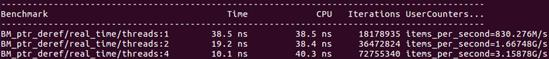
\includegraphics[width=0.9\textwidth]{content/2/chapter6/images/5.jpg}\\
图6.5 - 发布指针(消费者线程)的性能
\end{center}

结果应该与对原始指针的解引用进行比较,在多线程中也可以这样做:

%\hspace*{\fill} \\ %插入空行
\begin{center}
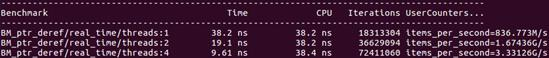
\includegraphics[width=0.9\textwidth]{content/2/chapter6/images/6.jpg}\\
图6.6 - 原始指针的性能,与图6.5进行比较
\end{center}

性能数据非常接近。还可以比较发布的速度,但消费者端更重要。每个对象只发布一次,然后进行多次访问。

了解发布指针不做什么同样重要。首先,在指针的构造中没有线程安全问题。假设生产者和消费者线程共享对构造好的指针,这个指针初始化为空。谁来构造并初始化了指针?在数据结构中,都有一个\textit{根指针},通过它可以访问整个数据结构,它由构造初始数据结构的线程初始化。还有一些指针,可作为某些数据元素的根,本身包含在另一个数据元素中。现在,想象一个简单的单链表,其中每个元素的“next”指针是下一个元素的根,而头是整个链表的根。生成链表元素的线程必须将“next”指针初始化为空。然后,另一个生产者可以添加一个新元素并发布。注意,这偏离了数据发布后就不可变的规则。但是,这里可以这样做,因为对线程安全\texttt{unique\_ptr}的更改都是原子的。无论如何,没有线程可以在指针构造的时候进行访问非常关键(这是一个非常常见的限制,大多数构造都不是线程安全的,因为对象在构造之前不存在,所以不能保证)。

指针没有做的事是,没有为多个生产者线程提供同步。如果两个线程试图通过同一个指针发布新数据,结果是未定义的,并且存在数据竞争(一些消费者线程将看到一组数据,而其他线程将看到不同的数据)。如果有多个生产者线程操作特定的数据结构,必须使用一种机制进行同步。

最后,虽然指针实现了线程安全的发布协议,但没有执行安全的“取消发布”和删除数据。它是拥有指针的,因此当删除时,所指向的数据也会删除。但消费者线程可以使用删除之前获得的值。数据所有权和生命周期的问题都必须处理。理想情况下,程序中应该有一个点,在这个点上,知道整个数据结构或不再需要某个子集了。消费者线程都不应该访问这些数据,甚至不应该保留指向它的指针。此时,\textit{根指针}和其指向的内容就可以安全的删除例如。在执行过程中如何安排,就是是另外一件事情了,通常由算法控制。

有时,希望指针能够以线程安全的方式同时管理数据的创建和删除。本例中,我们需要一个线程安全的共享指针。

\hspace*{\fill} \\ %插入空行
\noindent
\textbf{原子共享指针}

如果不能保证程序中有已知的点可以安全地删除数据,就必须清楚有多少消费者线程持有有效的数据指针。如果想要删除这个数据,必须等到在整个程序中只有一个指针指向它时,再安全地删除数据和指针本身(或至少将其重置为空)。这是进行引用计数共享指针的工作模式,计算有多少指向同一对象的指针,在没有对该指针的引用时,将该指针删除。

讨论线程安全的共享指针时,理解指针需要什么保证非常重要。C++标准共享指针\texttt{std::shared\_ptr}通常是线程安全的。如果多个线程操作指向同一对象的不同共享指针,那么对引用计数器的操作是线程安全的,即使两个线程导致计数器同时改变。若一个线程正在复制它的共享指针,而另一个线程正在删除它的共享指针,并且在这些操作开始之前引用计数是N,计数器将上升到N+1,然后回到N(或先下降,然后上升,中间值可以是N+1或N-1,但不存在数据竞争,并且行为很明确,包括最终状态。这个保证意味着引用计数器上的操作是原子的。实际上,引用计数器是一个原子整数,实现时使用\texttt{fetch\_add()}对其进行原子递增或递减。

只要没有多个线程共享同一个共享指针,这个保证就适用。如何获得每个线程自己的共享指针是另外一个问题,因为所有指向同一对象的共享指针必须以第一个指针的方式进行创建,这些指针必须在某个时间点从一个线程传递到另一个线程。假设,复制共享指针的代码受到互斥锁的保护。如果两个线程访问同一个共享指针,那么所有的猜测都是多余的。若一个线程试图复制共享指针,同时另一个线程正在重置它,结果是未定义的。特别是,标准共享指针不能用于发布协议的实现。然而,当共享指针的副本分发到线程(可能处于锁定状态)中,共享的所有权就会得到保护,对象的删除将以线程安全的方式处理。当最后一个指向该对象的共享指针删除时,该对象也会删除。请注意,由于每个特定的共享指针都会由一个线程处理,所以这是完全安全的。如果在程序执行期间,只有一个共享指针拥有对象时,那么也只有一个线程可以访问这个对象。其他线程不能复制这个指针(不让两个线程共享同一个指针对象),并且没有其他方法可以获得指向同一个对象的指针,所以删除操作将以单线程的方式进行。

这种方式很好,但两个线程会访问同一个共享指针呢?这种访问的例子就是发布协议。消费者线程正在读取指针的值,而生产者线程可能正在修改它,这样就需要共享指针本身的操作是原子的。在C++20中可以这样做,这里允许写\texttt{std::atomic<std::shared\_ptr<T>>}。注意,早期的建议写一个新类代替\texttt{std::atomic\_shared\_ptr<T>}。不过,这也不是最终的方法。

如果没有兼容C++20的编译器和相应的标准库,或者不能在代码中使用C++20的话,仍可以在\texttt{std::shared\_ptr}上执行原子操作,但需要显式地做。为了使用在所有线程之间共享的指针\texttt{p\_}发布对象,生产者线程必须这样做:

\begin{lstlisting}[style=styleCXX]
std::shared_ptr<T> p_;
T* data = new T;
… finish initializing the data …
std::atomic_store_explicit(
	&p_, std::shared_ptr<T>(data), std::memory_order_release);
\end{lstlisting}

另一方面,为了获得指针,消费者线程必须这样做:

\begin{lstlisting}[style=styleCXX]
std::shared_ptr<T> p_;
const T* data = std::atomic_load_explicit(
	&p_, std::memory_order_acquire).get();
\end{lstlisting}

与C++20原子共享指针相比,这种方法的主要缺点是无法避免非原子访问。开发者应该记住始终使用原子函数来操作共享指针。

虽然方便,但\texttt{std::shared\_ptr}并不是一个特别有效的指针,并且原子访问使它变得很慢。可以比较上一节中使用线程安全的发布指针和使用显式原子访问共享指针发布对象的速度:

%\hspace*{\fill} \\ %插入空行
\begin{center}
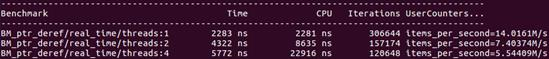
\includegraphics[width=0.9\textwidth]{content/2/chapter6/images/7.jpg}\\
图6.7 - 原子共享发布指针的性能(消费者线程)
\end{center}

同样,应该将这些数字与图6.5中的数字进行比较。发布指针在一个线程上要快60倍,而且这种优势会随着线程的数量变多而增加。当然,共享指针的意义在于提供了共享资源的所有权。因此,共享指针需要更多的时间来完成更多的工作。比较的重点是显示这种共享所有权的成本。如果可以避免,程序的效率会更高。

即使需要共享所有权(如果没有共享所有权,有些并发数据结构很难设计),使用有限的功能和最实现设计自己的引用计数指针,则可以完成得更好,一种常见的方法是使用侵入引用计数。侵入式共享指针将其引用计数存储在指向的对象中。当为特定对象(如特定数据结构中的列表节点)设计时,对象在设计时需要考虑到共享所有权,并包含引用计数器。否则,可以对任何类型使用包装器类,并使用引用计数器进行扩展:

%\hspace*{\fill} \\ %插入空行
\noindent
\textbf{04\_intr\_shared\_ptr\_mbm.C}
\begin{lstlisting}[style=styleCXX]
template <typename T> struct Wrapper {
	T object;
	Wrapper(… arguments …) : object(…) {}
	~Wrapper() = default;
	Wrapper (const Wrapper&) = delete;
	Wrapper& operator=(const Wrapper&) = delete;
	std::atomic<size_t> ref_cnt_ = 0;
	void AddRef() {
		ref_cnt_.fetch_add(1, std::memory_order_acq_rel);
	}
	bool DelRef() { return
		ref_cnt_.fetch_sub(1, std::memory_order_acq_rel) == 1;
	}
};
\end{lstlisting}

当减少引用计数时,要知道何时达到0(或在减少之前是1),共享指针就会删除对象。

即使是最简单的原子共享指针的实现也相当冗长,本章的示例代码中可以找到一个非常简单的示例。同样,这个示例只包含指针正确执行几个任务所需的最小值,例如:发布对象和多个线程并发地访问同一个指针。这个例子的目的是让我们更容易理解实现这类指针所需的基本元素(即使这样,代码也有几页长)。

除了使用侵入式引用计数器外,特定于应用的共享指针可以放弃\texttt{std::shared\_ptr}的其他特性,例如:许多应用程序不需要弱指针。一个极简的引用计数指针可以比标准指针高效几倍:

%\hspace*{\fill} \\ %插入空行
\begin{center}
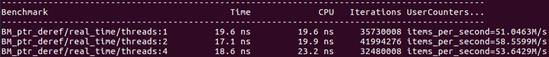
\includegraphics[width=0.9\textwidth]{content/2/chapter6/images/8.jpg}\\
图6.8 - 自定义原子共享发布指针(消费者线程)的性能
\end{center}

同样,对于指针的赋值和重赋值、两个指针的原子交换以及指针上的其他原子操作,它的效率更高。这个共享指针比唯一指针的效率低得多,若可以显式地管理数据所有权,则不需要引用计数。

现在,我们了解了数据结构的两个关键构建块,可以添加新数据并发布它(向其他线程显示),并需要跟踪其所有权,甚至是跨线程(这需要付出巨大代价)。




















